\documentclass[11pt,oneside,a4paper,english]{article}
\usepackage[T1]{fontenc}
\usepackage[utf8]{inputenc}
%\usepackage[latin2]{inputenc}
\usepackage[margin=2.25cm,headheight=26pt,includeheadfoot]{geometry}
\usepackage[danish, english]{babel}
\usepackage{listings}
\usepackage{color}
\usepackage{titlesec}
\usepackage{titling}
\usepackage[framed, numbered]{matlab-prettifier}
\usepackage{changepage}
\usepackage{amsmath}
\usepackage{hyperref}
\usepackage{enumitem}
\usepackage{graphicx}
\usepackage{fancyhdr}
\usepackage{lastpage}
\usepackage{caption}
\usepackage{tocloft}
\usepackage{setspace}
\usepackage{multirow}
\usepackage{titling}
\usepackage{float}
\usepackage{comment}
\usepackage{booktabs}
\usepackage{indentfirst}
\usepackage{lscape}
\usepackage{booktabs,caption}
\usepackage[flushleft]{threeparttable}
\usepackage[english]{nomencl}
\usepackage{xcolor}
\usepackage{lipsum}
\usepackage{biblatex}
\addbibresource{document.bib}
\usepackage{booktabs}
\usepackage{float}
%\usepackage[]{apacite}

% --- set footer and header ---
\pagestyle{fancy}
\fancyhf{}

\setlength{\parindent}{2em}
\title{CDIO 3} % to reference as \title, dont use \maketitle
\makeatletter\let\Title\@title\makeatother



\lstset{language=Matlab,
style=Matlab-editor,
basicstyle=\normalsize\mlttfamily,
numbers=left,
numberstyle={\scriptsize\color{black}},			% size of the numbers
numbersep=0.5cm											
}

\newlist{steps}{enumerate}{1}
\setlist[steps, 1]{leftmargin=1.5cm,label = Step \arabic*:}
\renewcommand{\headrulewidth}{1pt}
\renewcommand{\footrulewidth}{1pt}

%\lhead{\Title}
\rhead{\nouppercase{\rightmark}}
\lhead{\Title}
\rfoot{
\includegraphics[height=1.25cm]{images/logo.pdf}} % right header logo
\setlength\headheight{16pt}
\setlength{\footskip}{50pt}
\lhead{\Title} %rightH title
\cfoot{\thepage}

% --- End of page settings ---
%
%
%
%
%
%
% --- Start på dokument ---

\begin{document}
\pagenumbering{roman} 

\begin{titlepage}
\begin{center}
\vspace{2cm}
%\textsc{ Danmarks Tekniske Universitet}\\[1.5cm]

\includegraphics[width=0.4\textwidth]{images/dtu.png}~\\[1cm]
\vspace{2cm}

\vspace{2cm}

% Title
\hrule
\vspace{.5cm}
{ \huge \bfseries CDIO3} % title of the report
\vspace{.5cm}

\hrule
\vspace{1.5cm}

\textsc{\textbf{Forfattere}}\\
\vspace{.5cm}
\centering

% add your name here
Marcus Kastrup Ottosen - s205348\\
Frederik Nissen - s205332\\
Jean Bora Yagan - s205863\\
Rasmus Jehn Pedersen - s205257\\
Victor Kongsbak - s205363\\
Villads Hellman Andersen - s205349\\

\vspace{1cm}

\textsc{\textbf{Vejleder}}\\
\vspace{.5cm}
\centering
Mikkel Johansen - s175194


\vfill

\centering \today % Dags dato
\end{center}
\end{titlepage}
    % Viser forsiden

\newpage
\label{ch0.1}
\section*{Timeregnskab}

Alt timeregnskab er angivet i minutter.\\
Aflevering af opgave er sket Fredag uge 48.
\begin{table}[H]
\centering
\begin{tabular}{@{}lccccccc@{}} %c = center
\toprule
Uge 45   & Mandag & Tirsdag & Onsdag & Torsdag & Fredag & Lørdag & Søndag \\ \midrule
Frederik &    &    &    &  80  &    &    &    \\
Jean     &    &    &    &  80  &    &    &    \\
Marcus   &    &    &    &  80  &  30  &  30  &    \\
Rasmus   &    &    &    &  80  &    &    &    \\
Victor   &    &    &    &  80  &    &    &    \\
Villads  &    &    &    &      &    &    &    \\ 
\end{tabular}

\begin{tabular}{@{}lccccccc@{}}
\toprule
Uge 46   & Mandag & Tirsdag & Onsdag & Torsdag & Fredag & Lørdag & Søndag \\ \midrule
Frederik &  140  &  120  &    &    &    &    &    \\
Jean     &  140  &  120  &    &    &    &    &    \\
Marcus   &  140  &  100  &    &    &    &    &    \\
Rasmus   &  140  &  120  &    &    &    &    &    \\
Victor   &  140  &  120  &  60  &    &    &    &    \\
Villads  &    &   120 &    &    &    &    &    \\ 
\end{tabular}

\begin{tabular}{@{}lccccccc@{}}
\toprule
Uge 47   & Mandag & Tirsdag & Onsdag & Torsdag & Fredag & Lørdag & Søndag \\ \midrule
Frederik &    &    &    &    &    &    &    \\
Jean     &    &    &    &    &    &    &    \\
Marcus   &  180  &  60  &    &  120  &  300  &  70  &    \\
Rasmus   &    &    &    &    &  300  &    &    \\
Victor   &    &    &    &    &  300  &  70  &    \\
Villads  &    &    &    &    &    &    &    \\ 
\end{tabular}

\begin{tabular}{@{}lccccccc@{}}
\toprule
Uge 48   & Mandag & Tirsdag & Onsdag & Torsdag & Fredag & Lørdag & Søndag \\ \midrule
Frederik &  180  &    &    &    &    &    &    \\
Jean     &  40  &    &    &    &    &    &    \\
Marcus   &  270 &    &    &    &    &    &    \\
Rasmus   &  270 &    &    &    &    &    &    \\
Victor   &  270 &    &    &    &    &    &    \\
Villads  &    &    &    &    &    &    &    \\ \bottomrule
\end{tabular}
\caption{Timeregnskab}
\end {table}

\clearpage


\section*{Resumé}
\lipsum[3] 


\newpage
\tableofcontents    %Printer table of contents
\setstretch{0.95}



%figur-og tabelliste
\newpage
\addcontentsline{toc}{section}{Figurliste}
\listoffigures

\bigskip
%\newpage
\addcontentsline{toc}{section}{Tabelliste}
\listoftables



\newpage
\pagenumbering{arabic} 
\fancyfoot[C]{Page \thepage\ of \pageref{EndOfText}}


%kapitler
\newpage
\label{ch1}
\section{Indledning}
huhhu
\\
huhuh
\lipsum[1]
 

\newpage
\label{ch2}
\subsection{Funktionelle krav}
\subsubsection{Opsætning}
\begin{enumerate}
  \item Spillerne skal kunne lande på et felt og så fortsætte derfra på næste slag. 
  \item Felterne er opbygget så spillerne går i ring på brættet.
  \item Spillet skal kunne spilles af 2 til 4 personer.
  \item Alle spillere skal starte med et antal penge
  ({\rotatebox[origin=c]{180}{\textwon}}).
  
  \begin{enumerate}
      \item Ved 2 spillere skal hver spiller have 20 {\rotatebox[origin=c]{180}{\textwon}}.
      \item Ved 3 spillere skal hver spiller have 18 {\rotatebox[origin=c]{180}{\textwon}}.
      \item Ved 4 spillere skal hver spiller have 16 {\rotatebox[origin=c]{180}{\textwon}}.
  \end{enumerate}
  
  \item Spillet skal tage brug af en GUI
  \begin{enumerate}
      \item Spillet skal i starten have et input felt, hvor brugeren skal angive antal personer.
      \item Derefter skal spillet skal kun have 1 knap, som bruges til kast af terningen.
      \item GUI'en skal vise hver spillers pengebeholdning.
      \item GUI'en skal vise spillepladen med de forskellige felter og priser.
      \item GUI'en skal vise, hvor de enkelte spillere befinder sig på spillepladen.
      \item GUI'en skal vise, hvilke felter de enkelte spillere ejer.
  \end{enumerate}
  \item Alle felter der kan købes, skal have en pris fra 1 til 4 {\rotatebox[origin=c]{180}{\textwon}}.
\end{enumerate}



\smallskip
\subsubsection{Spilregler}
\begin{enumerate}
    \item Hver spiller kaster én terning, og rykker med uret rundt det antal felter på pladen, som øjnene viser.
    \item Hver gang der landes/passere start, modtager den enkelte spiller 2 {\rotatebox[origin=c]{180}{\textwon}}.
    \item Landes der på et ikke-ejet felt, skal spilleren købe det.
    \item Landes der på et felt der allerede er ejet, skal spilleren betale feltets værdi. Ejes feltet af samme spiller, gøres intet.
    \item Landes der på et felt der allerede er ejet, og ejeren også ejer den anden ejendom i samme farve, fordobles beløbet der skal betales.
    \item Hvis en spiller lander på "gå i fængsel" feltet, bliver spilleren flyttet til fængselsfeltet uden at passere start. Derudover mister spilleren sin næste tur, og bliver derfor sprunget over en hel omgang.
    \item Hvis man lander på et "chance" felt, bliver et chancekort trukket.
    
    \item Spillet slutter når en modstander er gået fallit. 
    \item Når spillet slutter findes vinderen, som er den spiller med flest {\rotatebox[origin=c]{180}{\textwon}}.
\end{enumerate}



\bigskip



\subsection{Ikke funktionelle krav}
\begin{enumerate}
\subsubsection{Visuelt}
    \item GUI'en skal have en høj grad af visualitet og brugervenlighed
    \begin{enumerate}
        \item Det skal være nemt for alle spillere, at finde ud af, hvordan de interagerer med spillet.
        \item Det skal være nemt for brugerne, at trykke på knappen.
        \item Brugerne skal tydeligt kunne se, hvor mange {\rotatebox[origin=c]{180}{\textwon}} de har.
        \item Det skal være tydeligt for alle spillere at se, hvor samtlige spillere befinder sig på pladen.
        \item Det skal være tydeligt for brugeren at se, hvor mange {\rotatebox[origin=c]{180}{\textwon}} hver grund koster.
        \item Det skal være tydeligt for brugeren at se, hvilke grunde er til salg.
    \end{enumerate}
    \item 
    
\end{enumerate}
 

\newpage
\label{ch3}
\section{Analysedokumentation}
    \subsection{Use Cases}
        \begin{enumerate}
          \item Start spillet
        \begin{itemize}
          \item Brugerne har mulighed for, at starte og slutte spillet. Evt. vha. vinduets knapper.
        \end{itemize}
         \item Kast terning
        \begin{itemize}
           \item Brugerne kan trykke på en knap for at kaste terningen.
        \end{itemize}
         \item Før spillets start, angiver brugeren antal spillere i et tekst-felt.
        \end{enumerate}
        
        
        \subsubsection{Use Case Diagram}
        
        \begin{figure}[H]
            \centering
            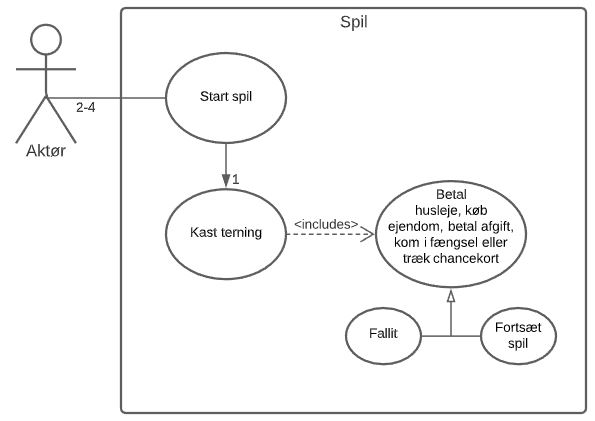
\includegraphics[width=10cm]{figures/usecase.jpg}
            \caption{Use Case Diagram}
            \emph{ Use Case Diagrammet viser hvordan en spiller interagerer med spillet}
        \end{figure}

            

            
        \begin{table}[H]
        \centering
        \begin{tabular}{|p{0.3\linewidth} | p{0.6\linewidth}|} 
        \hline
        \textbf{Name}                         &\textbf{ Kaste terninger}  \\ 
        \hline
        Short description                     & Hver spiller har muligheden for at trykke på knappen og dermed kaste en terning\\ 
        \hline
        Precondition                          & For at en terning kan kastes, kræves det at spillet er i gang, og brugeren er klar til at starte sin tur\\ 
        \hline
        Postconditions                        & Terningerne viser et antal øjne og spilleren kan nu rykke til det ramte felt. Spillerens tur er nu slut.\\ 
        \hline
        Error situation                       & Spilleren var ikke klar til at kaste terningerne og dermed starte sin tur.\\ 
        \hline
        System state in the event of an error & Hvis en spiller ved fejl kaster terningerne, vil spillet stadig fortsætte uden mulighed for at vende tilbage.\\ 
        \hline
        Actors                                & Spiller 1 og 2.\\ 
        \hline
        Trigger                               & Knappen til kast af terning bliver trykket på af en af spillerne. \\ 
        \hline
        
        Standard process                      & 
        \begin{enumerate}
        \item Terningen får en tilfældig værdi mellem 1-6.
        \item Spilleren bliver rykket frem på spillepladen svarende til terningens værdi ud fra spillerens position.
        \item Der skal betales husleje svarende til feltets værdi.
        \end{enumerate}
        \\ 
        \hline
        
        Alternative processes                 &                  
        \begin{enumerate}
        \item Terninger viser en værdi mellem 1-6.
        \item Spilleren bliver rykket frem på spillepladen og lander på feltet \textit{fængsel}
        \item Spilleren er nu i fængsel og modtager ikke 2 {\rotatebox[origin=c]{180}{\textwon}} ved passering af start.
        \item Der skal betales 1 {\rotatebox[origin=c]{180}{\textwon}} for løsladelse af fængslet.
        \end{enumerate}
        \\
        \hline
        
        
        
        
        
        
        \end{tabular}
        \caption{Fully Dressed Use Case Diagram}
        \end{table}
        
        \clearpage
        
        \subsubsection{Fully Dressed Use Case}
        \textbf{Navn}\\
        Kaste terninger.\\
        
        \textbf{Scope}\\
        Kaste terninger benyttes af spillerene til at spille spillet. Denne Use Case benyttes hver tur.\\
        
        \textbf{Level}\\
        Viser antal øjne.\\
        
        \textbf{Primære aktører og interessenter} \\
        Spillerne er primære aktører. Der er ingen interessenter.\\
        
        \textbf{Forudsætning} \\
        Der skal være 2 spillere som starter spillet. Hver spiller skal være klar til at starte sin tur og dermed kaste terningerne. Hver spiller skal slå med terningen for at få point.\\
        
        \textbf{Succeskriterier} 
        \begin{itemize}
            \item Spilleren kaster terningen og lander på et felt.
            \item Spilleren reagerer til feltet ved enten at købe ejendommen, betale huslejen eller betale afgiften. 
            \item Turen går videre til næste spiller, som gør det samme. 
        \end{itemize}
        
        \bigskip
        
        \textbf{Succes Scenarie (Main Flow)}
        \begin{itemize}
            \item Spilleren kaster en terning.
            \item Spilleren ser hvilket felt han/hun er landet på.
            \item Spilleren betaler husleje, afgift eller køber ejendom
            \item Turen går videre til den næste spiller
        \end{itemize}
        
        %systemsekvensdiagram
        \begin{figure}[H]
            \centering
            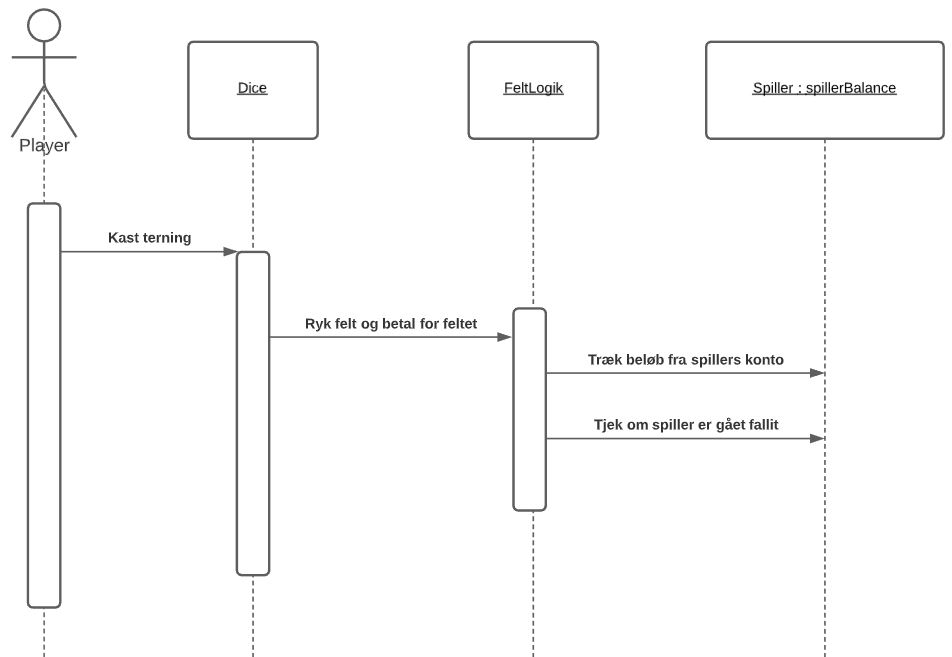
\includegraphics[width=14cm]{figures/systemSekvensDiagram.JPG}
            \caption{Systemsekvensdiagram}
            \emph{Systemsekvensdiagrammet viser step for step, hvilke handlinger spillet foretager. Dette Systemsekvensdiagrammet er tilføjet her for at illustrere et typisk succes scenarie ved brug af fully dressed use cases.}
        \end{figure}
        
        \textbf{Specielle krav} 
        \begin{itemize}
            \item Spillet skal åbnes af en spiller på en computer.
            \item Hver bruger kan fidne ud af at bruge en computer med en mus og keyboard.
        \end{itemize}
        
        \textbf{Frekvens}
        \begin{itemize}
            \item 
            \item
            
        \end{itemize}
        
        
    \subsection{Domæne model}
        \begin{figure}[H]
            \centering
            \includegraphics[width=14cm]{figures/domæneModel.JPG}
            \caption{Domæne model}
            \emph{Modellen her er en visualisering af hvordan matadorspillet fungerer i praksis}
        \end{figure}
    \subsection{System Sekvens Diagram}
        \begin{figure}[H]
            \centering
            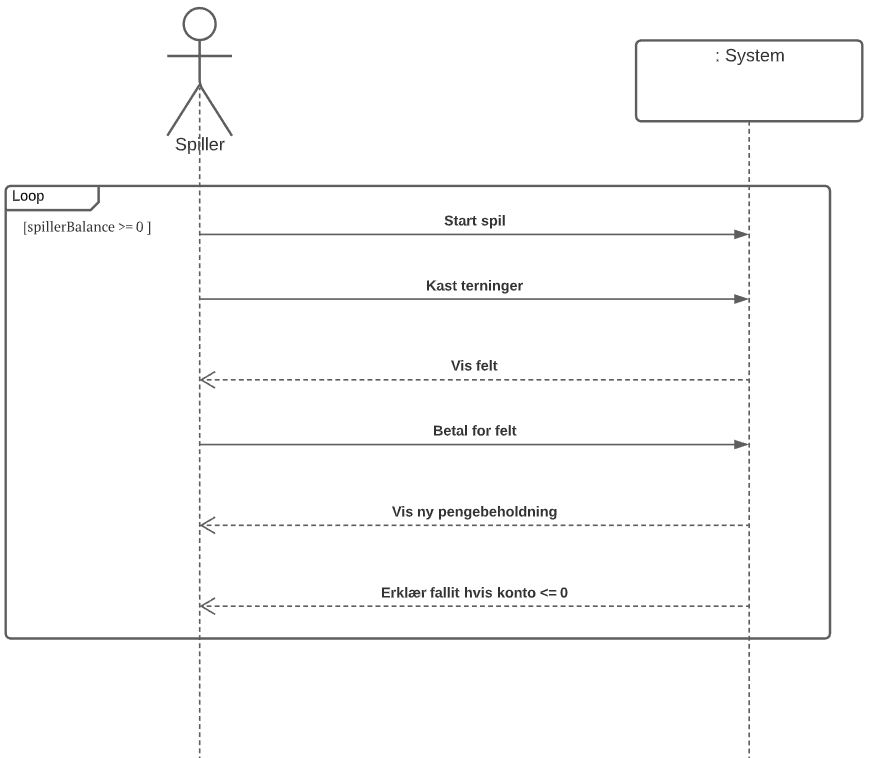
\includegraphics[width=14cm]{figures/overordnetSystemSekvensDiagram.JPG}
            \caption{Systemsekvensdiagram}
            \emph{Systemsekvensdiagrammet viser et overordnet billede af hvordan en aktør interagerer med systemet.}
        \end{figure}
        
    
    
    
 

\newpage
\label{ch4}
\section{Designdokumentation}
\subsection{Designklassediagram}
\begin{figure}[H]
            \centering
            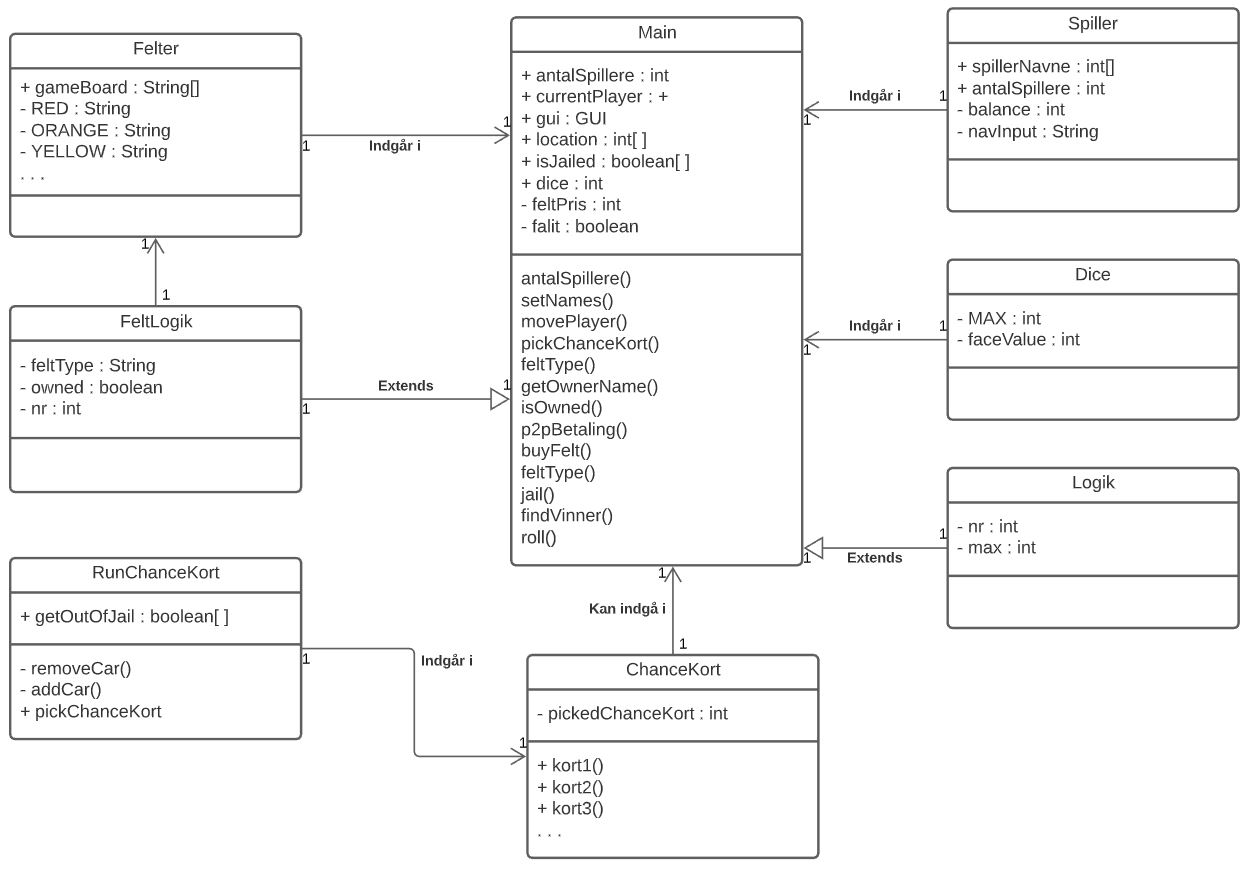
\includegraphics[width=14cm]{figures/designKlasseDiagram.JPG}
            \caption{Designklassediagram}
        \end{figure}
        
Design-klassediagrammet benyttes i alt sin simpelhed til at give et  hurtigt og overordnet overblik over systemets klasser og hvordan de er relateret til hinanden.  Klassediagrammet viser hvilke metoder og attributter der tilhøre den enkelte klasse, samt hvilke klasser der er associeret med hinanden. 
Ud fra klassediagrammet kan det ses, at der er en "Main" klasse, den klasse består af en længere række attributter som f.eks. antalSpillere, Gui, dice osv. Desuden er klassen tildelt samtlige metoder deriblandt, setName, movePlayer, feltType m.m. Main klassen er associeret med præcis 5 klasser, hvor netop Main indgår. Endvidere kan det ses at klasserne FeltLogik og Logik er nedarvet af Main, hvad også kaldes subclass og superclass. Det vil sige en klasse som kan gøre brug af variable fra den klasse, som den er nedarvet fra. 

Vi gør ikke brug af abstract klasser. En abstract klasse er en klasse, hvor metoderne er "låste" til klassen. Det kan bruges i situationer, hvor man ikke ønsker at metoderne skal kunne tilgås udefra klassen selv. 

Vi kunne også have gjort brug af polymorfi, da vi lavede felterne. Vi valgte dog at have alle felterne i en klasse, da vi vurderede, at det ikke ville fylde sønderligt meget. Ved brug af polymorfi kan man tilgå 2 metoder, som hedder det samme, fra 2 forskellige klasser og skelne imellem dem. 
        
\subsection{Sekvensdiagram}
    \begin{figure}[H]
        \centering
        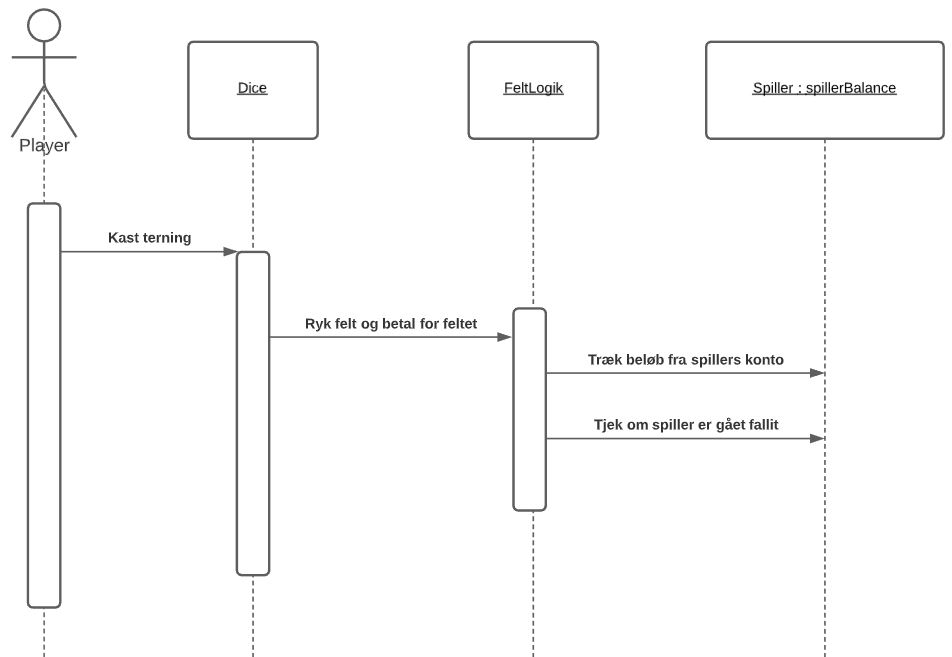
\includegraphics[width=15cm]{figures/systemSekvensDiagram.JPG}
        \caption{Sekvensdiagram}
        \emph{Sekvensdiagrammet illustrerer hvordan spillet virker som helhed}
    \end{figure}
    
Sekvensdiagrammet viser metodekaldene mellem forskellige objekter henover en arrangeret tidslinje. I diagrammet er der i øvrigt opmærksomhed på rækkefølgen, hvormed meddelelserne sendes til objekterne. 
Objekterne er illustreret ved lodrette streger som f.eks. "Kast terning" og "Træk beløb fra spillers konto", desuden viser den lodrette orientation også tiden. Hvert objekt sender meddelelserne fra et objekt til et andet, hvor der er givet en operation og et paramenternavn.  

\subsection{Brugergrænseflade}

Brugergrænsefladen er måden hvorpå brugeren benytter sig af systemet. Det er netop bindleddet mellem systemet og dets brugere. Der er særligt 2 punkter som brugergrænsefladen tilbyder; Inddata og uddata. Inddata tillader brugeren at styre systemet og uddata kan informere brugeren, også kaldt feedback. Disse former for data kan f.eks.vise brugernes kommandoer og systemets svar på de givne kommandoer. Dog er brugergrænsefladen helt principielt den facade brugeren har kontakt med som tastaturet og musen.

\newpage
\subsection{GRASP-mønstre}

I henhold til GRASP-mønstrene har vi forsøgt at overholde low coupling og high cohesion. Altså at koden er veldefineret i forhold til ansvarsområde, uden at være for afhængig af hinanden. Det har vi i spillet gjort ved at klasserne styrer hver deres del. Eksempelvis er Dice-klassen den samme som fra de foregående CDIO-projekter, med den éne arbejdsopgave, at stå for et tilfældigt output fra 1-6 

\newpage
\label{ch5}
\section{Implementation}
Matadorspillet er udelukkende skrevet i Java og vi har benyttet os af Intellij som IDE. Matadorspillet er opbygget af klasser, som vi har benyttet Java til at lave. \\
Der er tager brug af biblioteket Diplomitdtu:matadorgui version 3.1.7, hvilket GUIen er oprettet og bliver vist igennem. Da GUIen bliver fremvist ved hjælp af biblioteket, har vi, som programmører primært, skulle skrive logikken til spillet uden at fokusere på, hvordan det bliver vist for brugeren. Dette har vi gjort igennem 8 forskellige klasser, som sammen kommunikerer med biblioteket for at vi Matadorspillet til at fungere.
De forskellige klasser er forklaret nedenfor.\\
Et Javadoc til biblioteket kan findes i reference \cite{javadoc}. 
\\

\subsection{Spillets klasser}

\subsubsection{Main}
Main er en helt central klasse i programmet. Det er primært denne klasse som kommunikerer med GUIen. Derudover tager den brug af de fleste metoder fra de andre klasser. Da Main er så central i vores program, har vi valgt at oprette de fleste elementer, derunder variabler, arrays og objekter som public, så de kan tilgås fra de tilhørende klasser. Igennem kommunikation med biblioteket, bliver spillerne, spillepladen og felterne oprettet i Main.\\
I denne klasse bliver spillets primære loop også kørt. Loopet skifter mellem de forskellige spillere, og styrer bland andet hvornår en spiller skal kaste en terning, rykke og evt. betale eller medtage penge. Når dette loop bliver brudt, er spillet slut og en taber og evt. vinder vil findes.

\subsubsection{FeltLogik}
Feltlogik klassen er en public klasse, som extender mMin, for at kunne tilgå visse objekter oprettet i Main klassen. FeltLogik klassen bruges i sammenhæng med Main klassen til, at finde ud af, hvilket felt den enkelte spiller befinder sig på, tjekke hvorvidt feltet er ejet af en anden spiller, hvem der ejer det enkelte fag samt at rykke spilleren rundt på de forskellige felter. Derudover hjælper klassen også med, at rykke spilleren i fængsel, hvis spilleren har ramt feltet "Gå i fængsel". I klassen er der ingen variable som er oprettet til brug af hele klassen, men i stedet kun for de enkelte metoder. Variablerne er altså oprettet lokalt i de metoder som benytter dem.

\subsubsection{Spiller}
Spiller klassen har udelukkende forbindelse til Main klassen. Klassen holder styr på spillernes navne, antallet af spillere samt spillernes indledende balance. Klassen har 2 public variabler af hhv. et String array til spillernes navne, og en enkelt int til antallet af spillere. Disse to variabler er gjort public, da de begge bliver brugt inde i Main. Spiller klassen tager brug af bibliotekets GUI del, da der her bliver fremvist tekst-input felter til spillernes navne.

\subsubsection{Logik}
Logik klassen er en public klasse, som extender Main. Klassen extender Main, da klassen ikke ville kunne bruges eller fungere uden visse oprettede elementer i main, og det er derfor nødvendigt for Logik at Main findes. Denne klasse er blevet oprettet for, at fordele de mange metoder vores program tager brug af, ud i flere kategorier. Logik er altså klassen hvor de variabler som ikke gav mening af oprette inde i enten FeltLogik eller Spiller. Med Logik klassen er det muligt, at finde både vinder og taber samt køb af felt og betaling mellem to spillere.

\subsubsection{ChanceKort}
ChanceKort klassen er en meget simpel klasse, som bruges til at henvise videre til metoderne i RunChanceKort. Klassen er en public class hvis formål er, at finde et tilfældigt chancekort og initialisere metoden inde i RunChanceKort ved hjælp af en simpel switch.

\subsubsection{RunChanceKort}
RunChanceKort indeholder alle spillets chancekort, deres tekst og deres logik, og har mulighed for at fremvise chancekortne i GUIen når nødvendigt. Hvert chancekort er altså i stand til, at både rykke spillerne rundt på pladen, få spillere ud af fængslet samt give og trække penge på de respektive konti.

\subsubsection{Felter}
Felter klassen består udelukkende af et array af felterne på spillerpladen. Ved hjælp af det importerede matador bibliotek, bliver hvert felt oprettet som et objekt med en række variabler der kan angives ved start. Da denne klasse ikke på noget tidspunkt ændrer sig, er klassen oprettet som public final og dets variabler er oprettet som private final. Alle variabler i denne klasse er udelukkende brugt i klassen selv.

\subsubsection{Dice}
Dice klassen er en public klasse hvis formål er at kaste terningen og derved finde et random tal mellem 1 og 6. Hvis man ønsker at ændre terningen til en større type terning, kan dette nemt ændres ved at ændre klassens MAX værdi. Terningen bliver udelukkende brugt til, at angive hvor mange felter spilleren skal rykke på brættet.

 

\subsection{Versionsstyring}
Versionsstyring foregår igennem GIT ved brug af Github som fjern repository. Ved udvikling af dette projekt har vi benyttet os af flere branches til forskellige dele af projektet. Der er bl.a. blevet oprettet en \emph{udviklings branch}, som vi har benyttet til at skrive koden i. Når et stykke kode er skrevet i udviklings-branchen, har vi herefter oprettet \emph{Release branch}, hvor de forskellige dele af programmet samles sammen. Her testes der om programmet nu virker samlet og er dette tilfældet, bliver hele programmet merget ind \emph{master branch}, som nu danner baggrund for det færdig udviklet program.
\\Derudover er der også oprettet en \emph{feature branch}, som kan benyttes til at skrive ny kode og teste forskellige scenarier, som går ud over projektbeskrivelsen, uden at det har indflydelse på det færdig skrevet kode.

\begin{figure}[H]
        \centering
        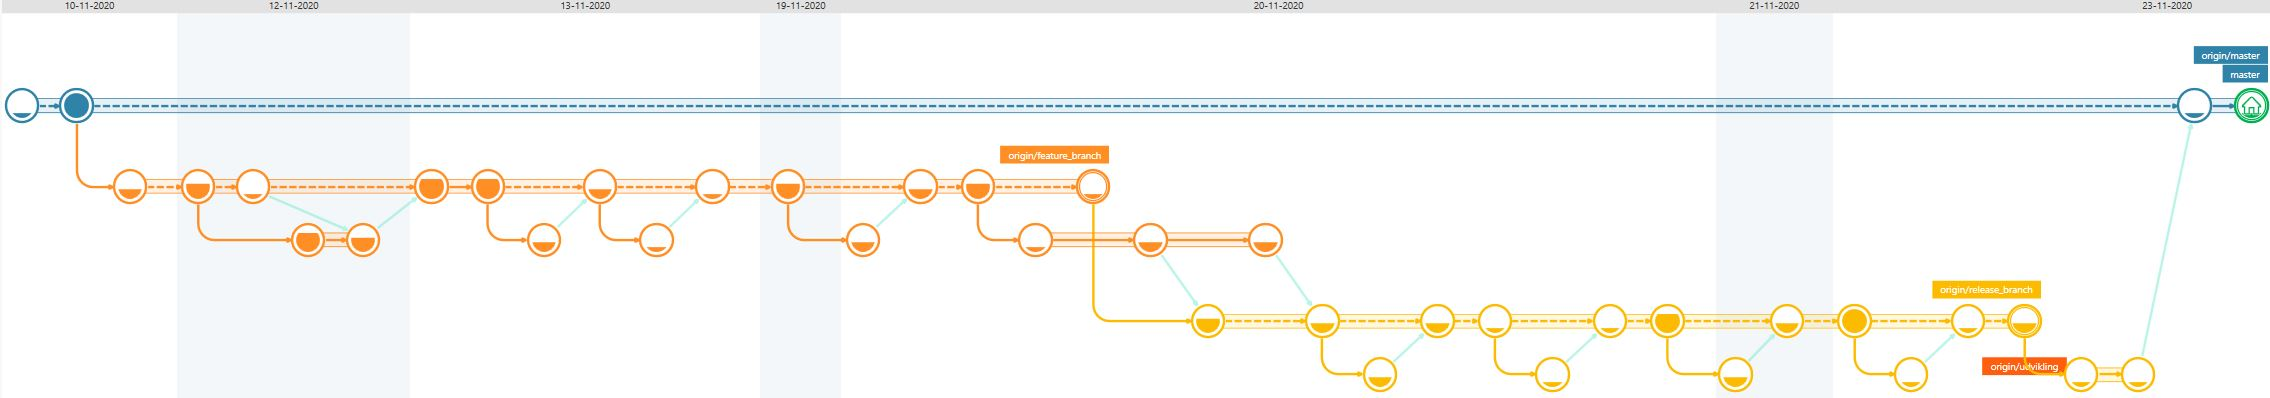
\includegraphics[width=17cm]{figures/gitVisualize.JPG}
        \caption{Git Visualization with GMaster}
    \end{figure}
     

\newpage
\label{ch6}
\section{Test}

%Lav mindst tre testcases med tilhørende fremgangsmåde/testprocedure og testrapporter.
%Lav mindst én Junit test til centrale metoder. Inkludér code coverage dokumentation.
%Lav mindst én brugertest. Husk at brugeren skal være en der ikke kan kode.

\subsection{Programtest}


\subsection{Brugertest}

\subsection{Test af terningens tilfældighed}
    \begin{figure}[H]
        \centering
        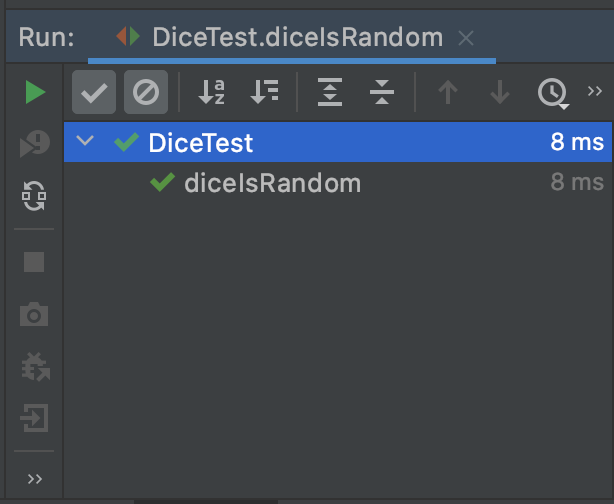
\includegraphics[width=8cm]{figures/diceIsRandomTest.png}
        \caption{JUnit test for at teste tilfældigheden af Dice klassens metode roll()}
        \emph{Testen af Dice klassen og dens roll() metode var en succes. Koden ses i bilag \ref{diceTest}}
    \end{figure}
    

\subsection{Test af chancekort tilfældighed}
    \begin{figure}[H]
        \centering
        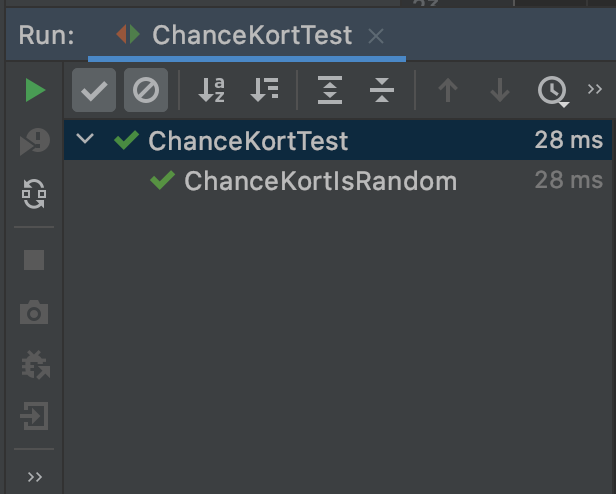
\includegraphics[width=8cm]{figures/chanceKortIsRandom.png}
        \caption{JUnit test for at teste tilfældigheden af ChanceKort klassens metode randomChanceKort()}
        \emph{Testen af ChanceKort klassen og dens randomChanceKort() metode var en succes. Koden ses i bilag \ref{ChanceKortTest}}
    \end{figure}
    
    
    \subsection{Test af antal chancekort}
    \begin{figure}[H]
        \centering
        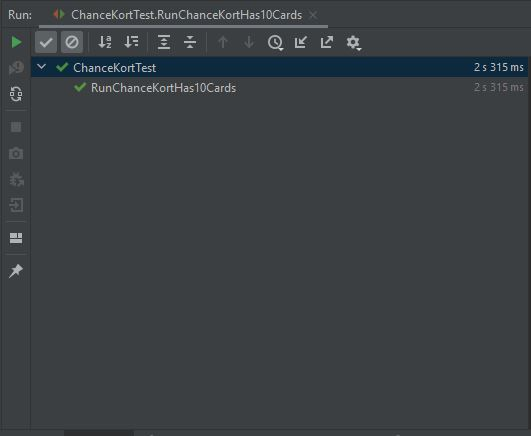
\includegraphics[width=15cm]{figures/RunChanceKortHas10Cards.JPG}
        \caption{JUnit test for at teste at RunChanceKort klassen indeholder det rigtige antal kort.}
        \emph{Testen af RunChanceKort klassen var en succes. Koden ses i bilag \ref{ChanceKortTest}}
    \end{figure}





 

\newpage
\label{ch7}
\section{Konfiguration}
Konfigurationen sætter en række krav til system, før at det færdigudviklede matadorspil kan køres på den valgte enhed. Derudover følges der op med en guide på kompilering, installation og afvikling fra GitHub, hvis der ikke ønskes at tage brug af den medfølgende .jar fil.

\subsection{Udviklingsplatform}
Vi har under udviklingen tager brug af programmet IntelliJ til udvikling af selve programmet. Heri er der hentet en håndfuld biblioteker for at gøre vores arbejde nemmere.\\
Til vores projektplanlægning har vi taget brug af online-værktøjet Trello, hvor alle har haft rettigheder til, at oprette rykke og fjerne planer.\\
Selve rapporten er udarbejdet udelukkende i LaTeX ved brug af Overleaf.

\subsection{Produktionsplatform}
\subsubsection{Hardwarekrav}
\begin{enumerate}
\item Enheden skal have mousepad, mus eller en touchskærm for at kunne interagere med programmet.
\item Minimum en Pentium 2 266 MHz processor.
\item En skærm større end 480p x 480p er nødvendigt, for at brugerne kan se hele GUI'en.
\end{enumerate}


\subsubsection{Softwarekrav}
\begin{enumerate}
\item UTF-8 skal være installeret på enheden.
\item Der skal være installeret Java JDK 14 på enheden.
\item Systemet skal have mindst 124 MB til rådighed på harddisken.
\item System skal køre Windows 10 20H2 eller macOS Mojave.
\end{enumerate}



\subsection{Vejledning til kompilering, installation og afvikling}
Importering fra Git: \\
I IntelliJ åbnes et nyt projekt fra “version control”. Som version control vælges “Git”, og følgende link til Github bruges:
https://github.com/marcusottosen/CDIO3. \\
Derefter skal kildekoden compiles ved at trykke på File -> Project Structure. \\
Under “artifacts” trykkes på plusset og der vælges JAR -> Create JAR from Modules.
Modules er “CDIO 3” og Main Class er “Main”.\\

Nu kan projektet compiles under Build -> Build Artifact, og vælge CDIO 3 -> Build. \\
I output-mappen findes nu en “CDIO 3.jar” som kan køres på maskiner med java installeret. \cite{CDIO2} 

\newpage
\label{ch8}
\section{Projektplanlægning}
\subsection{Uge 45}
I uge 45 begynder vi projektet, ved at gøre os nogle tanker om hvordan det hele skal bygges op. Det er her vi planlægger hvornår hvad skal laves, så vi alle er klar over hvor der skal startes.\\
Vi begynder allerede her at kigge på de første UML modeller, samt specificerer vores krav.

\subsection{Uge 46}
Uge 46 vil vi udarbejde diverse modeller til at beskrive programmet. Vi vil blandt andet udarbejde en domæne model, diverse sekvensdiagrammer og system sekvens diagrammer. \\
Her vil vi også udarbejde nødvendige use cases, der skal til for at leve op vores krav.\\
Vi begynder på første dele af vores program i denne uge. Vi vil begynde at udarbejde de forskellige klasser og teste dem ved brug af JUnit tests.

\subsection{Uge 47}
I uge 47 vil vi færdiggøre vores kode og udføre de sidste test. 

\subsection{Uge 48}
Sidste uge vil vi samle projektet og færdiggøre rapporten. Her vil vi merche alt koden sammen. 

 

\newpage
\label{ch9}
\section{Konklusion}
\subsection{Produkt}
Ved brug af den udleverede GUI har vi har fået udviklet et fungerende Monopoly-junior spil. Dette inkluderer alle de væsentlige ting fra det fysiske brætspil som spillernes figur, visuel terning, spillertransaktioner, fængsel og chancekort.

\subsection{Proces}
Inden opstart af projektet, fik vi i gruppen udarbejdet en gruppekontrakt. Denne kan findes i bilag \#2.
\\Til udviklingen brugte vi en udleveret GUI, som indeholdte meget af hvad, vi skulle bruge til spillet. Det er første gang, det har været fremgangsmåden, og har sådan set virket fint. Naturligvis krævede det, at vi lige skulle sætte os ind i dokumentationen for GUI'en. Det voldte dog heller ikke de store problemer.
\\
Dernæst har vi til rapportens udarbejdelse benyttet os af LaTeX i form af overleaf. Første indtryk var, at der ville være lidt af en indlæringskurve, hvilket også var tilfældet. Vi har styr på det mest grundliggende, men ved også, at der meget, som vi endnu mangler at få styr på. 
trel
\subsection{Perspektivering}
Selvom spillet kører som det skal med dets mest essentielle egenskaber, er der lige et par ting, som vi gerne ville have haft implementeret. Det er eksempelvis:
\begin{itemize}
\item Spiller vælger selv en unik brik-og farvekombination.
\item Få egne billeder og figurer visuelt vist på brættet.
\item Farven på huset på ejerens grunde matcher grundens ejer.
\item De resterende chancekort.
\item Dobbelt husleje hvis en pågældende spiller ejer begge felter af samme farve.
\item Landes der på et felt der allerede er ejet, og ejeren også ejer den anden ejendom i samme farve, fordobles beløbet der skal betales.
\item Hente alt tekst fra en txt. fil, så man nemt kan ændre eller oversætte spillet til et andet sprog.
\end{itemize}
 






\label{EndOfText}

\newpage
\pagenumbering{Roman} 
\fancyfoot[C]{Page \thepage\ af \pageref{endOfDoc}}

%-- Kildehenvisninger ---
\newpage
\printbibliography


%--- BILAG ---
\newpage
\label{bilag}
\section{Bilag}
\subsection{Test}
\subsubsection{Test a dice}\label{diceTest}
\begin{lstlisting}[language=Java, caption=Dice is random test]
import static org.junit.jupiter.api.Assertions.*;

public class DiceTest {
    

    /** Test af JUnit for at teste at det er sat korrekt op.
     * Her testes der blot om der er en konstruktør i Dice klassen */
    @org.junit.Test
    public void constructorExists() {
        Dice d1 = new Dice();
        assertEquals(Dice.class, d1.getClass());
    }


    /** diceIsRandom testen skal teste hvorledes metoden roll() i klassen Dice er tilfældig,
     * når den skal slå et tal fra 1-6 */
    @org.junit.Test
    public void diceIsRandom() {
        int diceRoll;
        int diceCount = 0;

        Dice d1 = new Dice();

        for (int i = 0; i < 100000; i++) {
            diceRoll = d1.roll();
            //Det antages at med 1 terning vil vi ca. få hvert slag 16.666 gange ud af
            //de 100.000 slag.
            if(diceRoll == 1) {
                diceCount++;
            }
        }

        //Vi tester om terningen slår 1. 16.666 gange, med 1% afvigelse
        if (diceCount < 16500 || diceCount > 16832) {
            fail("Terningen er ikke tilfældig, da den slog 1. færre eller flere gange end forventet");
        }
    }
}
\end{lstlisting}

\subsubsection{Test a ChanceKort}\label{ChanceKortTest}
\begin{lstlisting}[language=Java, caption=ChanceKort is random test]
import java.lang.reflect.Method;

import static org.junit.jupiter.api.Assertions.*;

public class ChanceKortTest {

    
    //Testen her er lavet på alle 24 kort, derfor fejler den nu, hvor der kun er 10 kort. Testen var en succes, da der var 24 kort. Dette ses også i rapporten.
    @org.junit.Test
    public void ChanceKortIsRandom() {
        int kort;
        int kortCounter = 0;

        ChanceKort kortTest = new ChanceKort();

        for (int i = 0; i < 1000000; i++) {
            kort = kortTest.randomChanceKort();

            //Det antages at ud af 24 kort er chancen for at trække kort 1. = 1/24
            //
            // Hvis vi trækker et kort 1.000.000 gange, bør vi få kort 1.
            // ca. 41.666 gange.
            if (kort == 1) {
                kortCounter++;
            }
        }
        System.out.println(kortCounter);
        //Nu tester vi om vi har trukket kort 1 det forventede antal gange
        //Vi tager hensyn til afvigelser, så vi tester med 1% afvigelse fra det forventede antal
        if (kortCounter < 41250 || kortCounter > 42082){
            fail("Du trak ikke kort 1. det forventede antal gange. Metoden er altså ikke tilfældig");
        }
    }

    @org.junit.Test
    public void RunChanceKortHas10Cards() throws ClassNotFoundException {
        //Expected er 12. 10 kort + 2 ekstra metoder, til at fjerne og tilføje biler.
        int expected = 12;
        int actual = 0;
        Class c = Class.forName("RunChanceKort");
        Method methods[] = c.getDeclaredMethods();
        for (int i = 0; i < methods.length; i++) {
            actual++;
        }
        assertEquals(expected, actual);
    }
}
\end{lstlisting}

\subsection{Gruppekontrakt}
\begin{figure}[H]
    \centering
    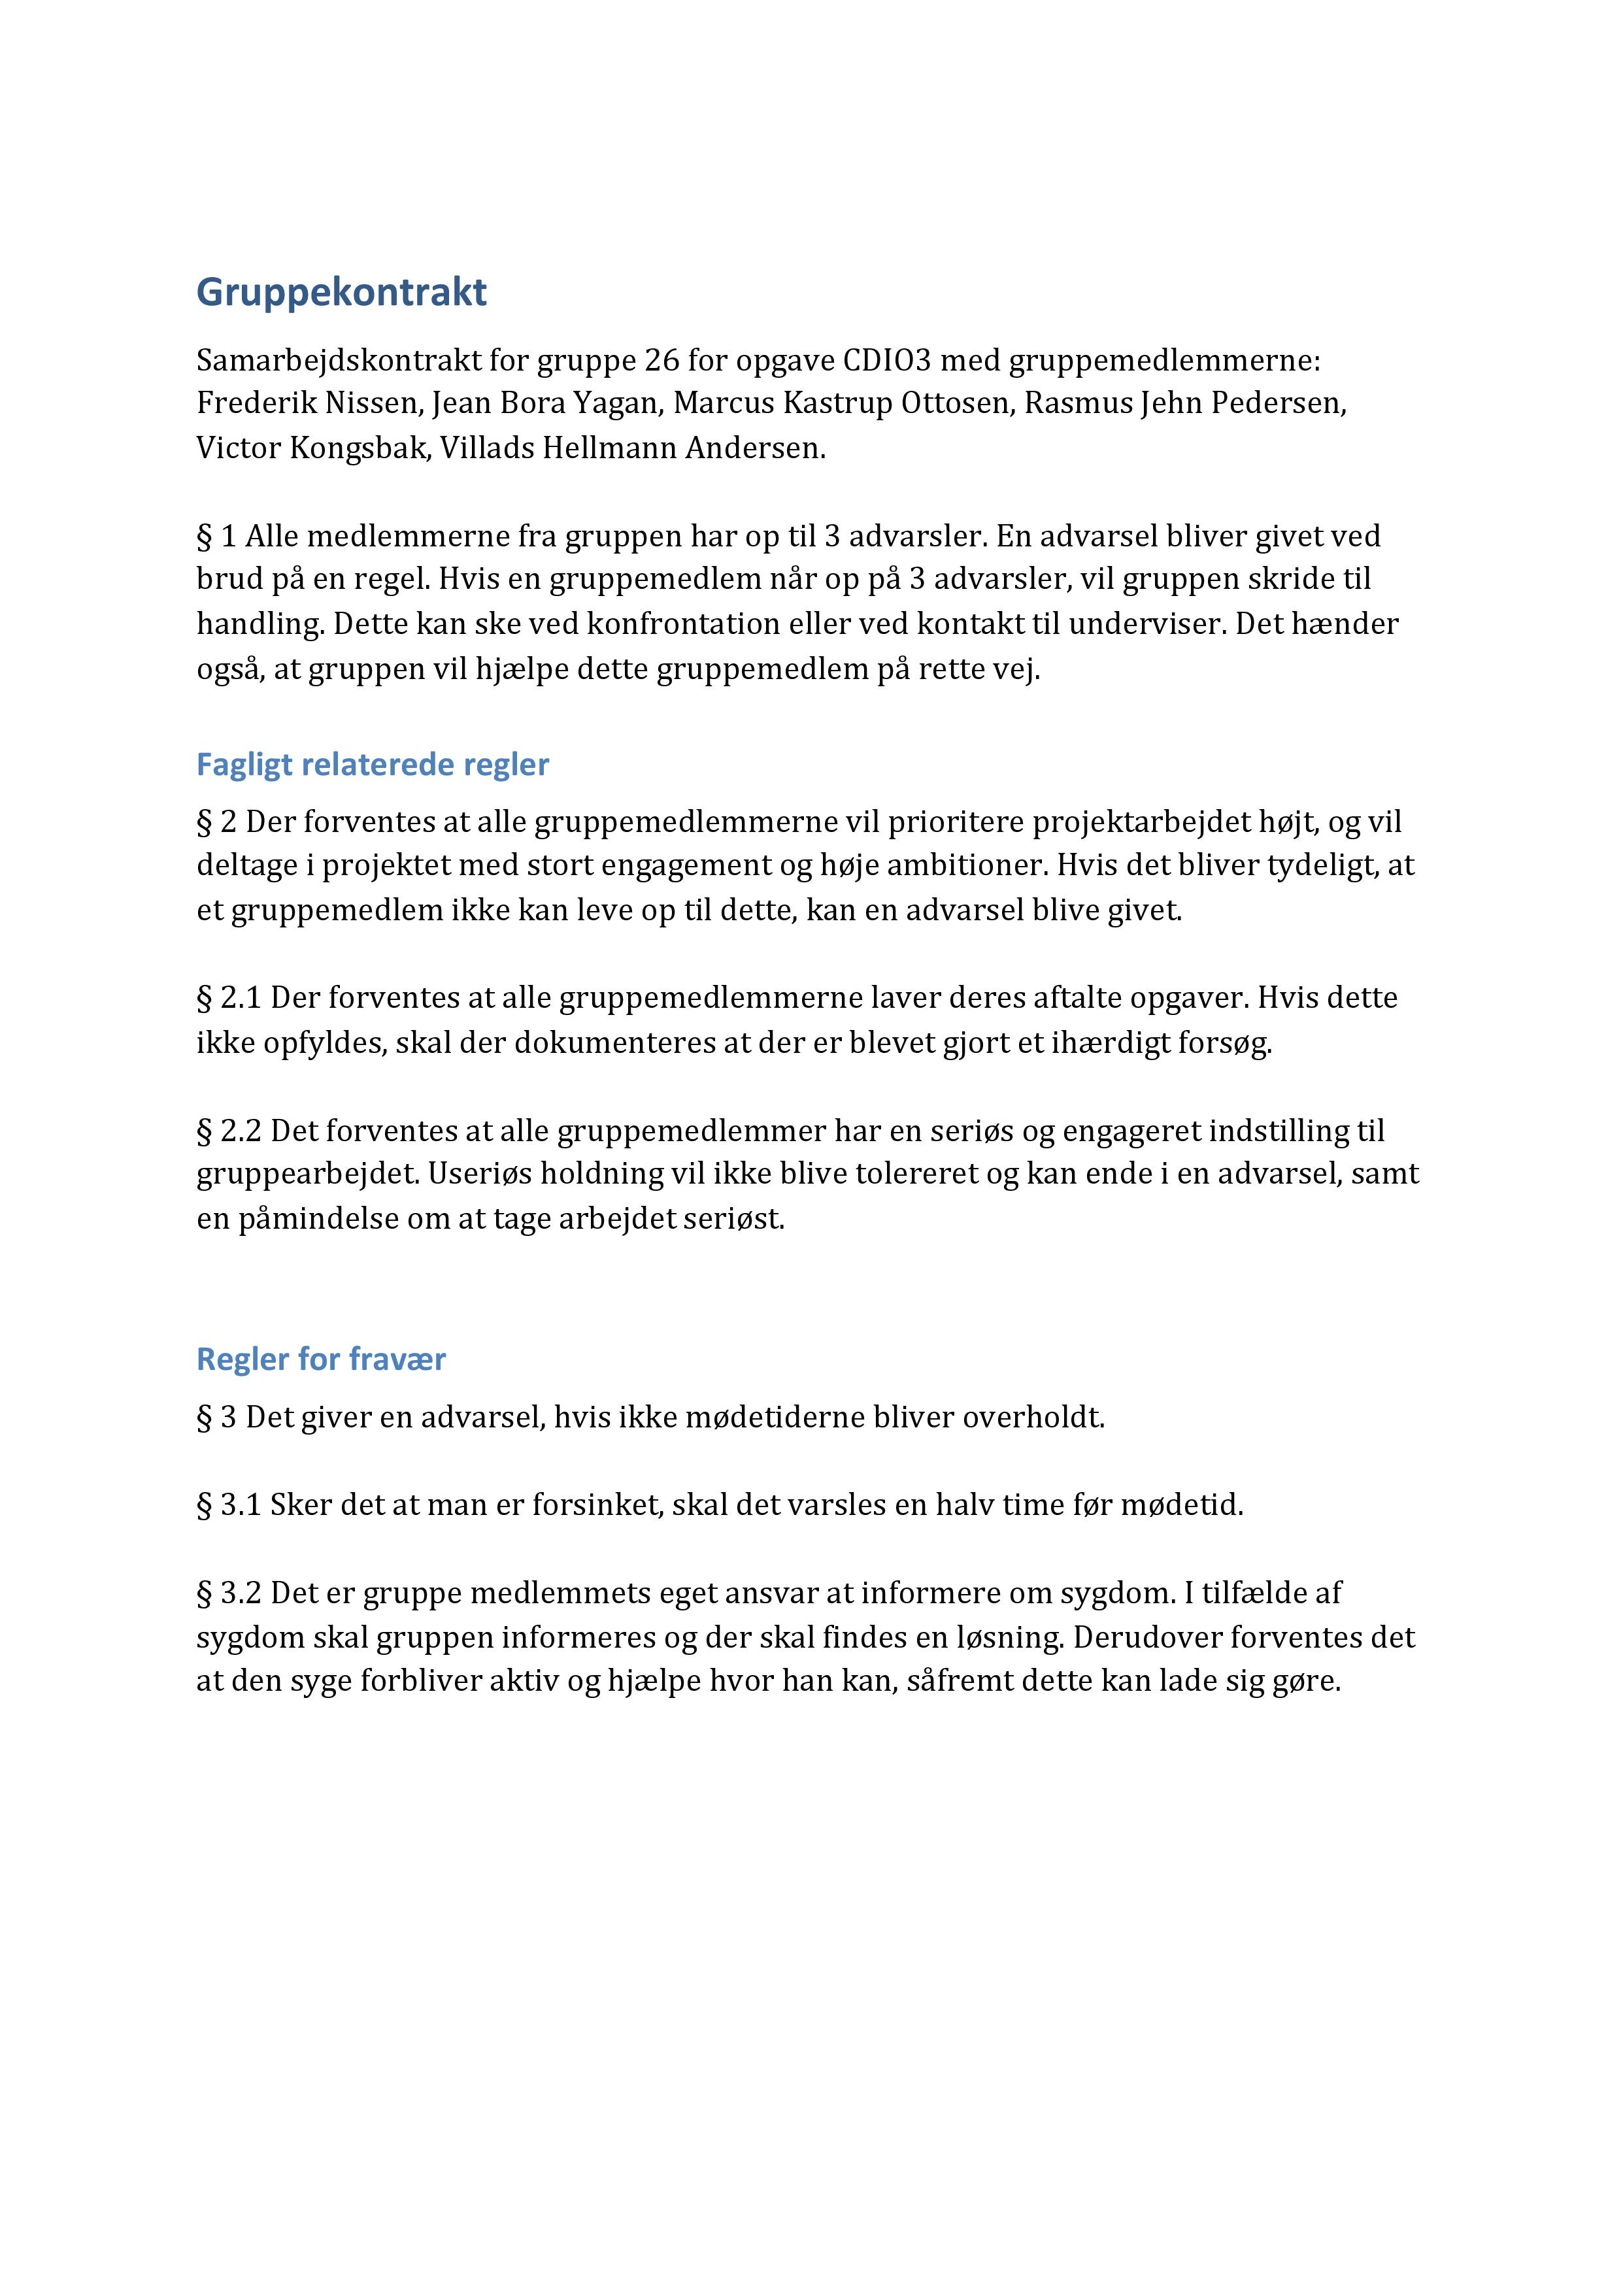
\includegraphics[width=17cm]{figures/Gruppekontrakt1.jpg}
\end{figure}
\begin{figure}[H]
    \centering
    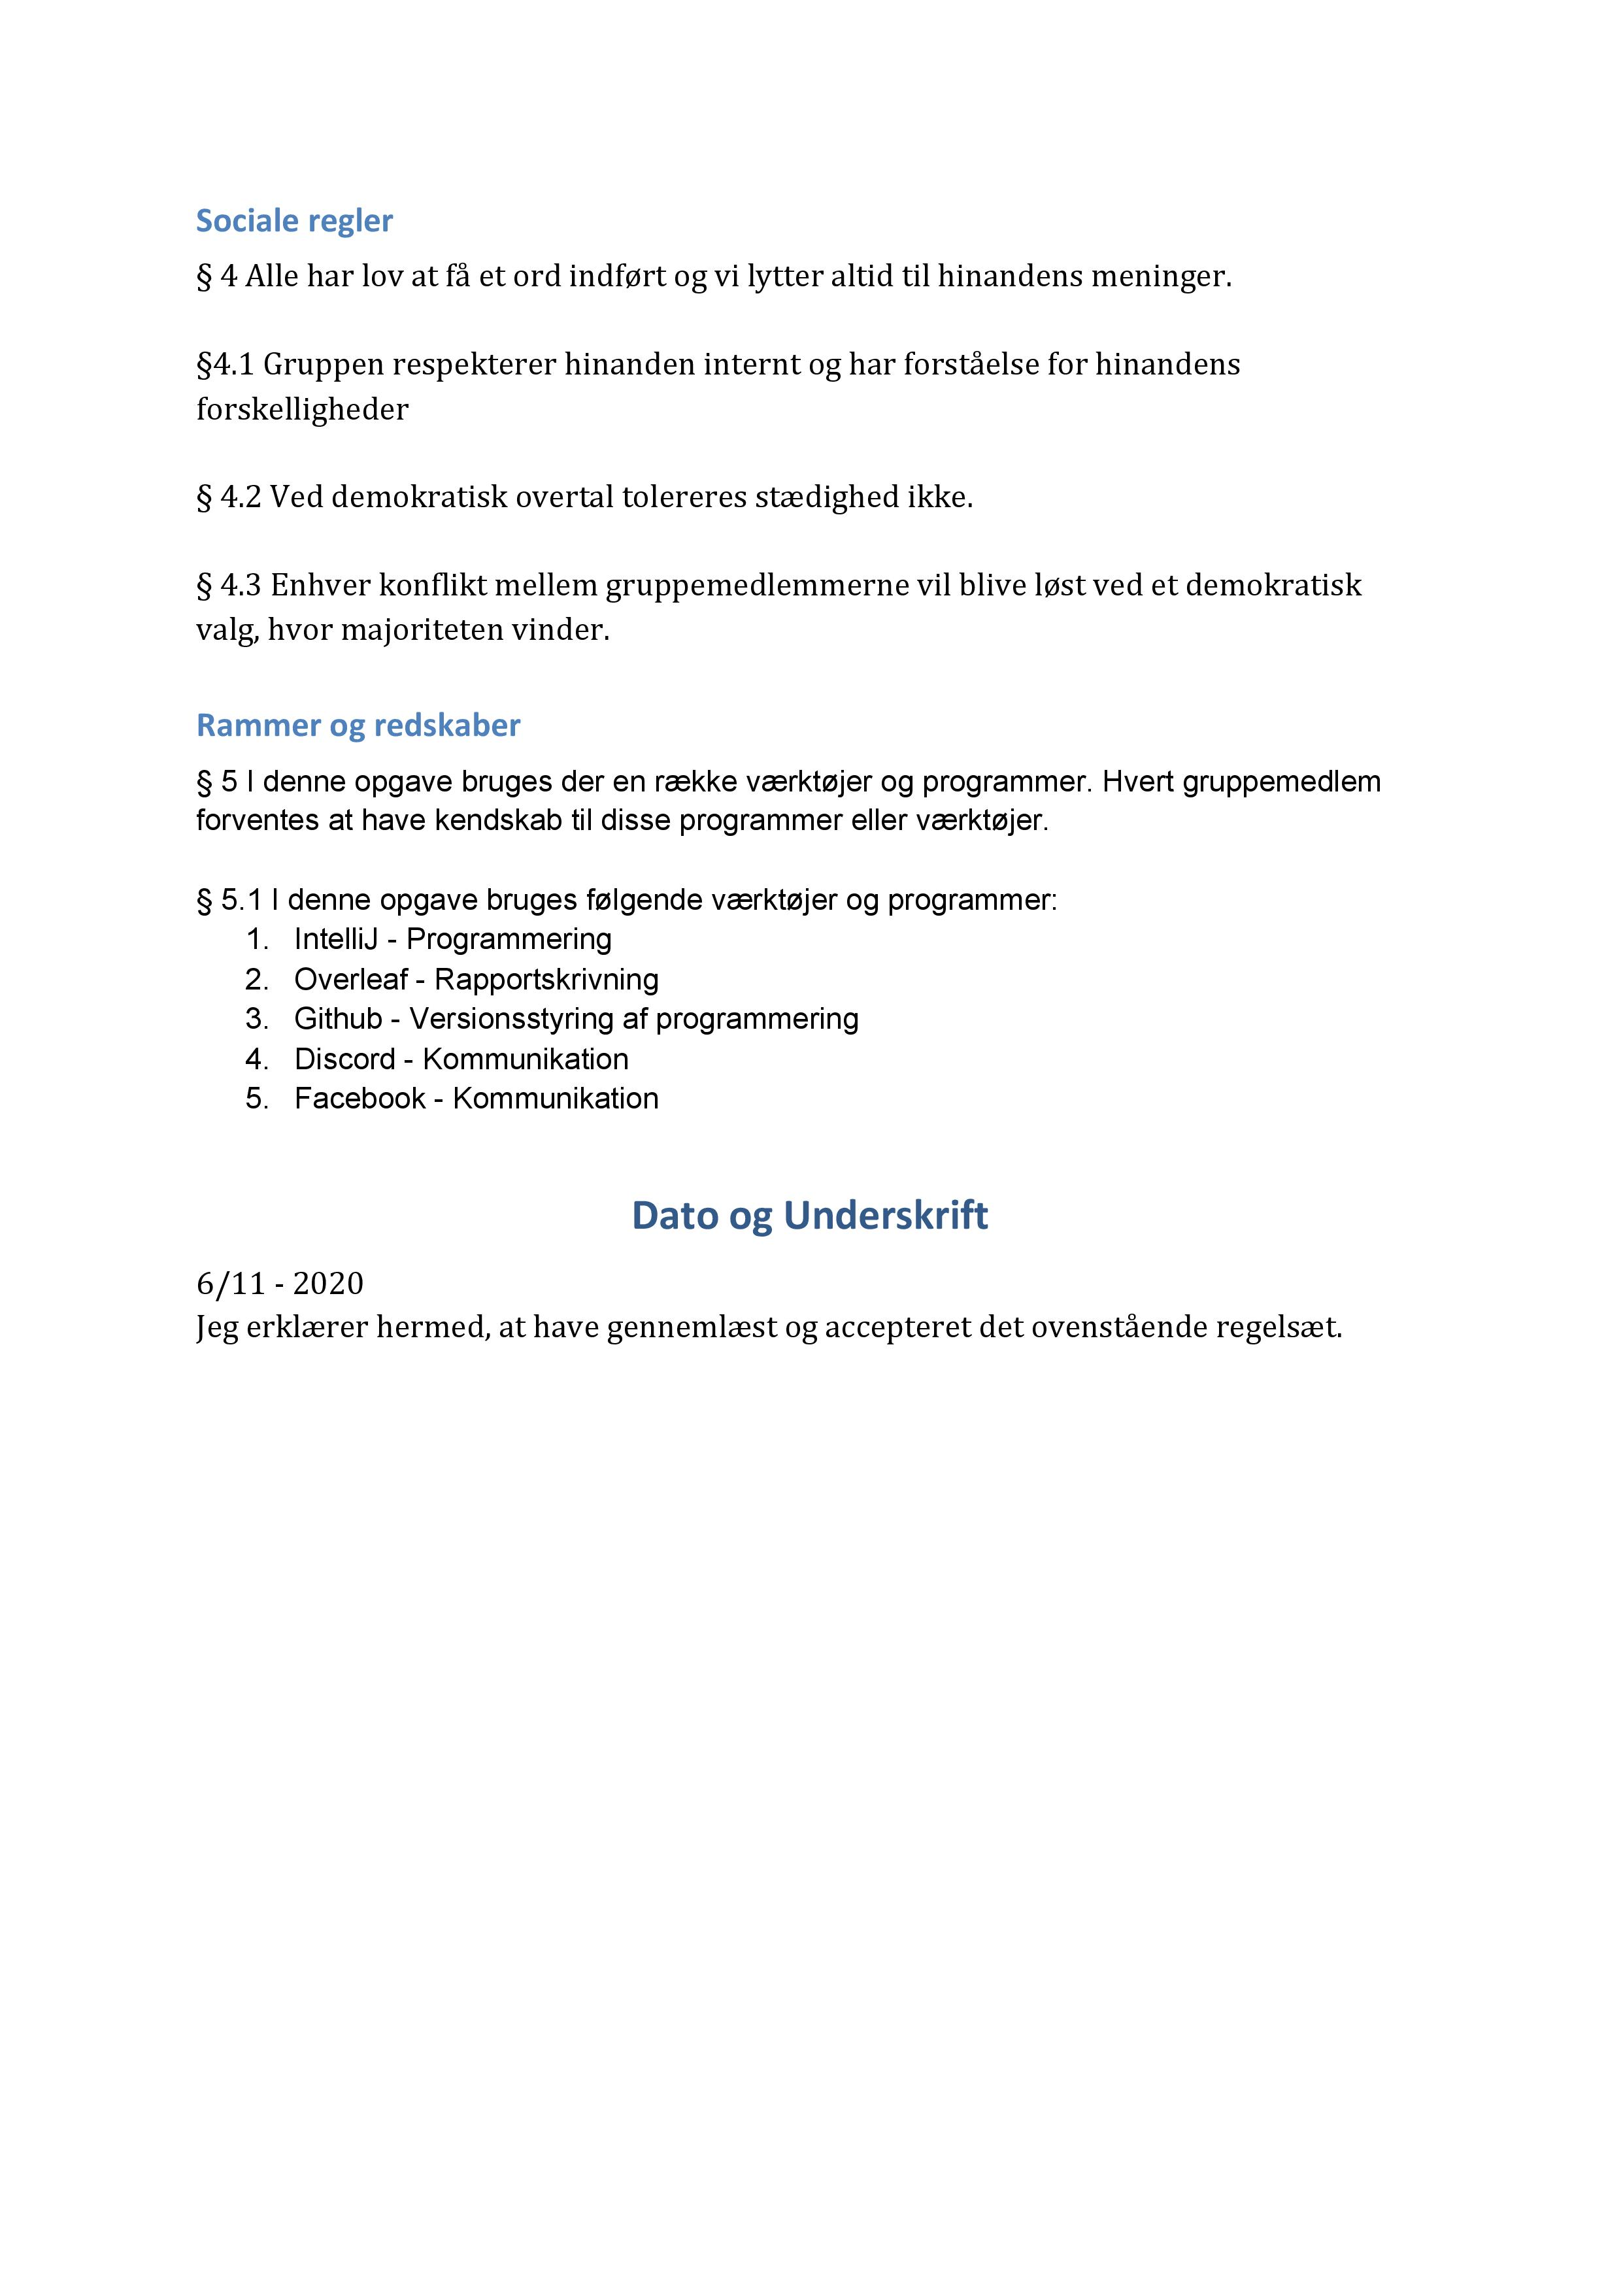
\includegraphics[width=17cm]{figures/Gruppekontrakt2.jpg}
\end{figure}

\label{endOfDoc}
\end{document}
